\chapter{State Space Analysis and Verification}
\label{chapter:analysis}

The state of a dynamic system refers to a minimal set of variables, called state variables, that fully describe the system and its response to any given set of inputs. This minimum set of variables, $s_i(t), i=0,1,2,..n$ along with knowledge of those variables at an initial time $t_0$ and the system inputs for time $t > t_0$, are sufficient to predict the future system state and outputs for all time $t > t_0$. This asserts that the dynamic behavior of a state is completely characterized by the set of state variables $s_i(t)$. 

CPN Tools uses a built-in \emph{state space} analysis tool to generate a bounded state space from an initialized CPN model. Here, the state space is a directed graph structure where the vertices, called states, each represent a unique system state. An edge between two states represents the transition from one state to another. If a state $S$ can non-deterministically transition into $K$ possible future states, then $S$ becomes the root of a K-ary tree. The state of the system in our case is a record of all the places in the CPN i.e. the token values in every place of the CPN model. This record is therefore a snapshot of the token configuration of the net and represents its execution state. State space generation is a process of generating this directed graph, from some initial state. State spaces of dynamic systems can be potentially infinite if there is always a potential unique state transition. For pragmatic reasons, we generate a bounded state space i.e. a graph structure bounded by some rule e.g. $t_i < t_bound$, where $t_i$ is some global time variable. In this case, the state space will contain only nodes where the state variable $t_i$ is less than some upper bound $t_{bound}$. Alternately, the rule can be to generate a state space as long as the component message queue size is under 50 waiting requests. 

To illustrate the state space analysis of DREMS using our CPN, we consider a simple example -- consider three equal-priority components, grouped into a process and executed on a single device. Each component has a periodic timer that fires every 10 ms and triggers the respective components into executing a block of code. Each component maps to an executor thread and these three threads are scheduled concurrently with all other threads in the system. In this example, there are no other component threads or system-level threads considered. Based on the OS scheduling scheme, these components, with equal priority, are scheduled using round-robin conflict resolution i.e. one of these threads is chosen at random and then a cyclic scheduling order is maintained. Since all three timers have the same period and the relative offsets are zero, the three timers fire concurrently and the respective component threads are marked as 'ready' at the exact same time. Since all three component threads are ready to execute the same times, there are $3!$ possible thread execution orders in the worst case when following round-robin scheduling. 

Figure \ref{fig:SSScreenshot} shows a bounded state space generated in CPN Tools for this component assembly. There are 6 branches from the initial state of the system as the model realizes the 6 possible behaviors. Each node in this state space is annotated with a state space ID and also a pair of integers in the format \emph{"p:c"}, where p refers to the number of parent nodes and c refers to the number of child nodes. This figure also shows results of a \emph{state space query}. Specifically, the query finds the \emph{marking} on the \emph{Completed\_Operations} place in two different state space nodes, 35 and 37. In node 37, Timer\_3\_operation is the first operation to complete as Component\_3 is the first ready thread chosen by the OS. In node 35, Timer\_1\_operation is the first operation to complete as Component\_1 is the first ready thread chosen by the OS. This illustrates the tree of possible behaviors that is encoded in the state space starting from an initial state. The goal of state space analysis is to search this tree of possibilities to identify a single execution trace i.e. a single branch in this tree that either satisfies or negates a system property e.g. that the deadline of one of these timer operations is violated. 


\begin{figure}[htb]
	\centering
	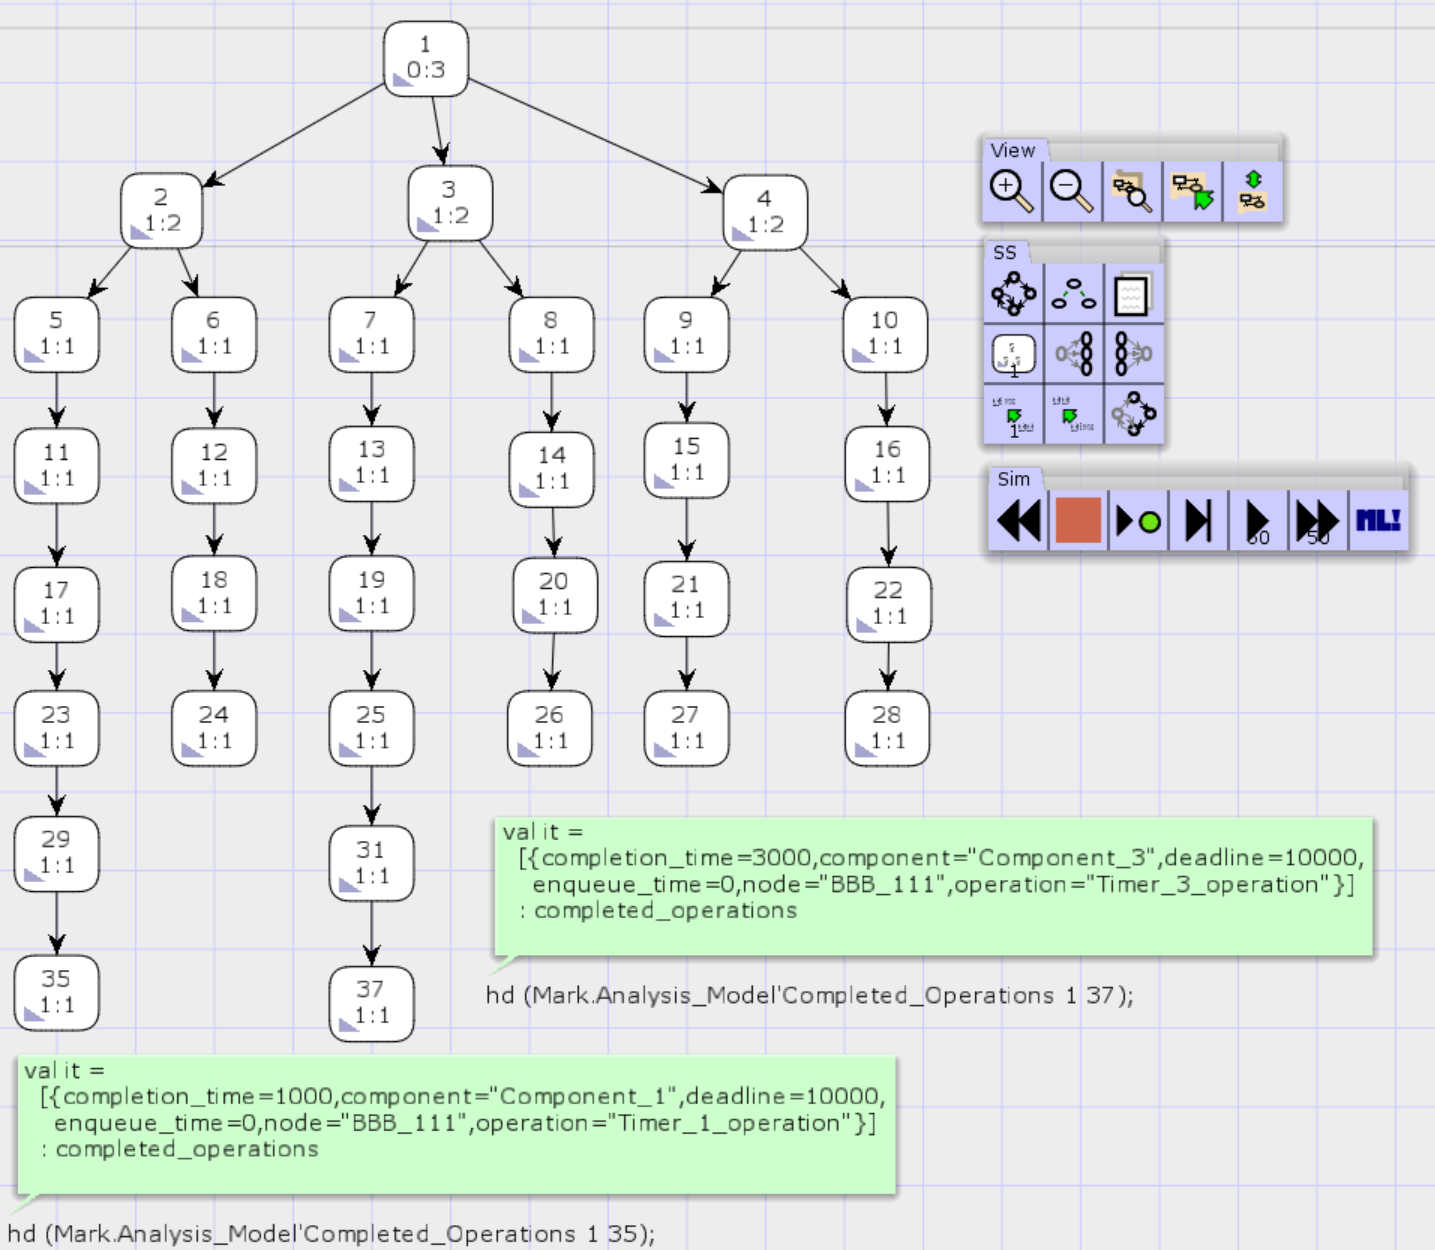
\includegraphics[width=\textwidth]{./img/state-space-analysis.png}
	\caption{Bounded State Space for a Multi-component Timer example -- The component threads have the same real-time priority and are executed in the same device. Each component is triggered with a 100 Hz periodic timer and all three timers are synchronized to illustrate non-determinism. The round robin  scheduling quantum is set to 4 milliseconds. 'Mark' is a state space query function that provides the \emph{marking} of a place in a particular state space node.}
	\label{fig:SSScreenshot}
\end{figure}
\FloatBarrier

\subsection{Searching the State Space}

CPNTools' inbuilt state space analysis tool comes with a programming interface -- a set of function that can be used by a user to query a generated state space. One of the many available functions is the \emph{SearchNodes} function, as shown in Figure \ref{fig:SSSearching}. This function traverses the nodes of the state space and at each node, evaluates a predicate and accumulates a list of nodes that satisfy this predicate. 

\begin{figure}[htb]
	\centering
	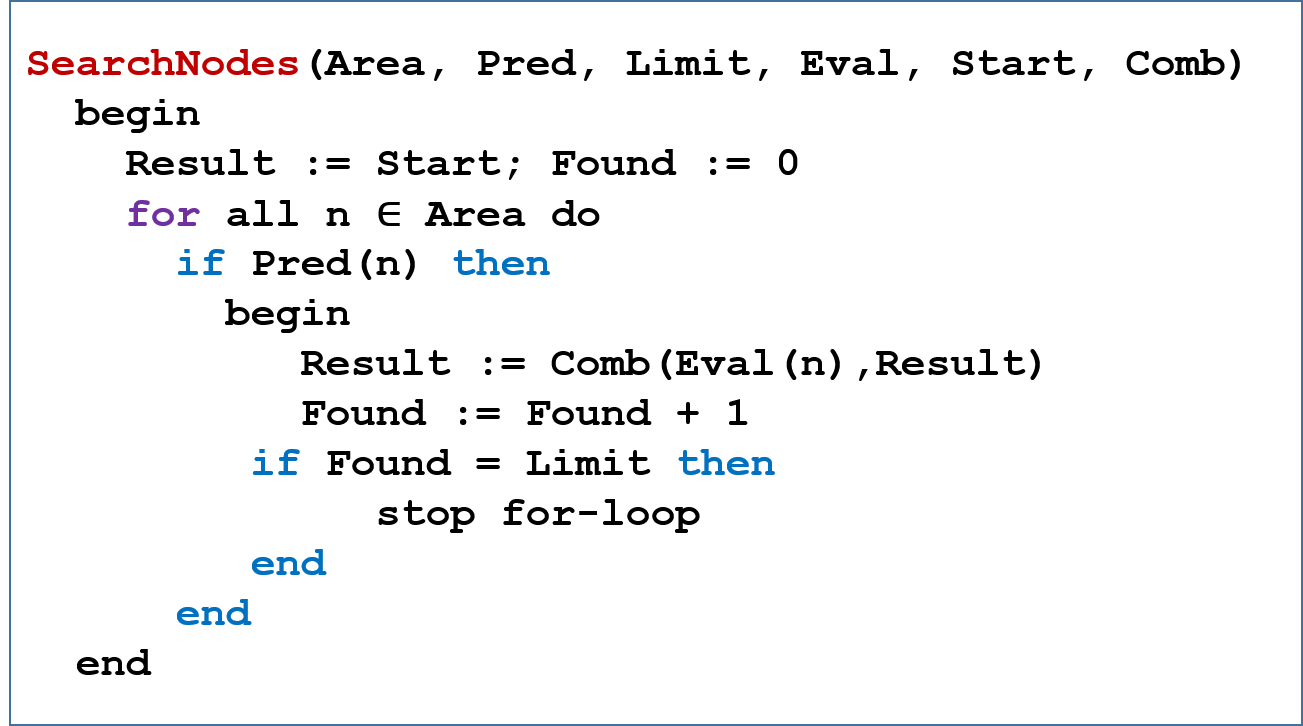
\includegraphics[width=0.7\textwidth]{./img/state-space-searching.png}
	\caption{SearchNodes function provided by CPNTools}
	\label{fig:SSSearching}
\end{figure}
\FloatBarrier

There are six parameters provided to this search function. \emph{Area} refers to the search area i.e. the part of the state space that needs to be searched. Often, the search area is the entire graph but it is possible to provide a subset of the graph e.g. a list of strongly connected components \footnote{A directed graph $G$ is strongly connected if every vertex is reachable from every other vertex in the graph. A strongly connected component is a maximal strongly connected subgraph of $G$ i.e. no additional edges or vertices from $G$ can be included in the subgraph without breaking its property of being strongly connected}. The second argument, emph{Pred}, specifies a predicate function that evaluates each node and produces a boolean result. All nodes that evaluate to false are ignored and all nodes that evaluate to true are retained for further analysis. The third argument, \emph{Limit} is an integer referring to how many times a predicate should evaluate to true before the search should terminate. If this limit is infinite, the entire state space is always searched. \emph{Eval} is an evaluation function that is executed on all state space nodes that satisfy the predicate function e.g. an evaluation function to find the execution time of an operation when its predicate function detects a deadline violation. Lastly, \emph{Start} is the initial value of the result and \emph{Comb} is a combination function that accumulates each new result from the evaluation function with prior results. The combination function is a constant time operation as it simply appends a new node to the end of the accumulated results list. The search algorithm itself has a time complexity of $O(n)$ where $n$ is the number of nodes in the state space. 

The rest of this chapter details how a bounded state space can be used to analyze DREMS applications for deadline violations, response times predictions etc. 

\subsection{Deadline Violations}

A \emph{deadline violation} refers to a system state where the execution time of a component operation has exceeded its deadline. The operation may violate its deadline without beginning execution since wait times in the message queue count towards the total delay from the arrival of the message to the completion of the corresponding operation. The SearchNodes function in CPNTools is quite generic and can be easily applied to our analysis model to identify such violations in the state space. For all operations, either completed or waiting for execution, it is sufficient to execute the predicate $current\_time - operation.enqueue\_time > operation.deadline$. All nodes that satisfy this predicate are nodes that represent deadline violation states. 

Alternatively, by adding observer places to our timing analysis model i.e. places that passively observe the system and accumulate tokens when certain conditional transitions execute, deadline violations can be recorded as the model is executing. A \emph{Deadline\_Violation} (Figure \ref{fig:DL}) transition fires at any point in time when the guard \emph{dl\_guard} is satisfied and arc bindings are realized with its input places. The transition observes the states of the currently running threads and the component message queues to identify deadline violations on operations that are either executing or waiting to execute. The \emph{dl\_violation} tokens in \emph{Late Operations} ($LO$) is of the form:

\begin{equation}
\label{eq:DLV}
LO = \ <Node_{name}, O_{name}, O_{ST}, \ O_{DLT}>
\end{equation}

where operation $O_{name}$ executing on computing node $Node_{name}$ started at time $O_{ST}$ and violated its deadline at time $O_{DLT}$. Since the component-level scheduler uses a non-preemptive scheme, this operation is still run to completion after the violated deadline. Delays like these propagate to the waiting operations in the message queue.

\begin{figure}[htb]
	\centering
	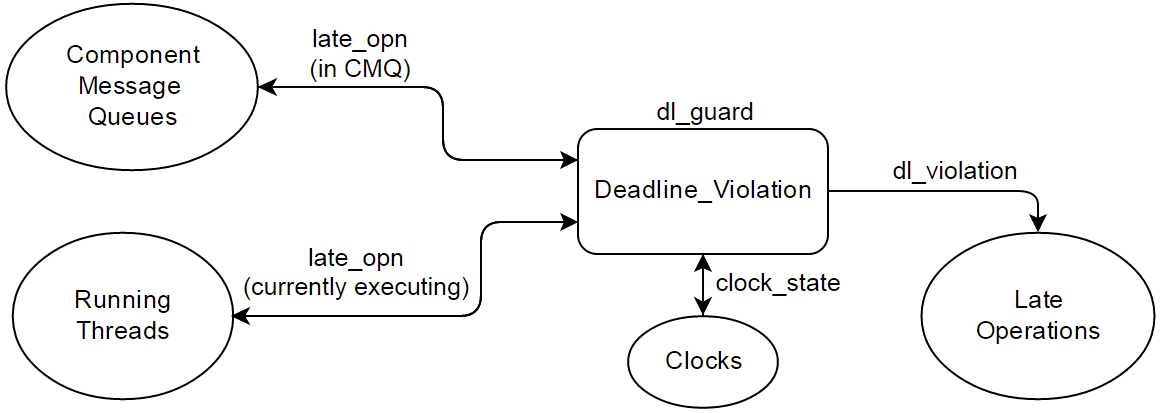
\includegraphics[width=\textwidth]{./img/Deadline_Violations.png}
	\caption{Deadline Violation Observer place}
	\label{fig:DL}
\end{figure}
\FloatBarrier

\subsection{System-wide Deadlocks}

System-wide deadlocks are caused by the inability of the OS schedulers (on all devices) to schedule any component executor thread. This can be caused by situations where a set of executing threads are indefinitely blocked on each other e.g. A server operation invoking an RMI on an already blocked client component. Such scenarios are typically due to cyclic dependencies that are undetected during system design. Using state space analysis such deadlocks can be detected in several ways.

One of the ways is to check if all of the component threads are blocked in any state space node i.e. the number of tokens in the place \emph{Blocked\_Threads} is equal to the total number of component threads. In CPNTools, this is expressed using the query as shown in Figure \ref{fig:blocked_threads}. This uses the SearchNodes function to search the entire state space graph and identify state space nodes where all component threads are blocked waiting on each other. The value SystemWideDeadlock is the resultant list of state space nodes where this predicate is true. Using nodes in this list, a trace can be generated to find the sequence of operations that lead to the deadlock. Using this trace, any implicit circular dependencies can be detected. 

\begin{figure}[htb]
	\centering
	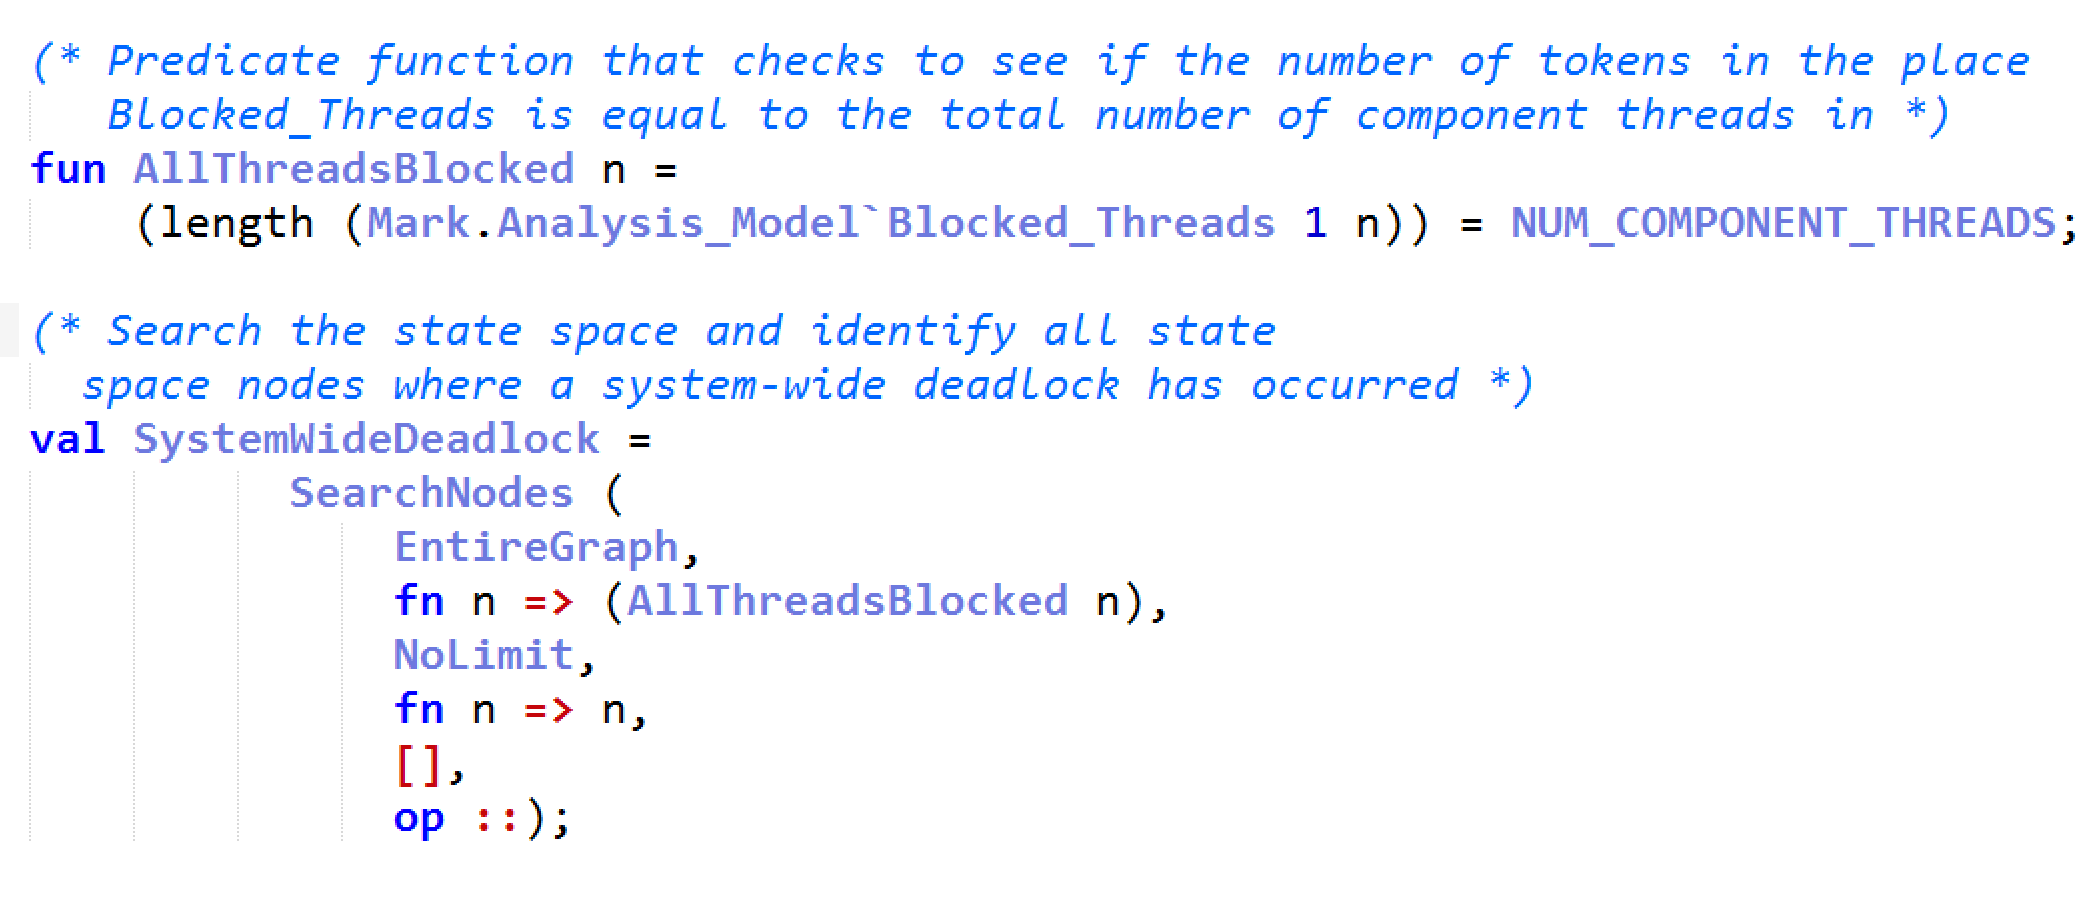
\includegraphics[width=\textwidth]{./img/blocked_threads.png}
	\caption{SML Query to detect system-wide deadlocks caused by (blocking) cyclic dependencies between components}
	\label{fig:blocked_threads}
\end{figure}
\FloatBarrier

\subsection{Response-time Analysis}

Response time analysis identifies the worst-case time taken for the system to generate a desired output signal after an input trigger has been provided e.g. time taken for the emergency braking system on an automated train controller to respond to sensory input. A component-based system can have a variety of triggers but in this context, a trigger is considered as any operation request received by a component. The response to this trigger is the completion of some other operation at a future time instant after the occurrence of the trigger. With state space analysis, it is possible to identify the worst-case response times for a $(trigger\_operation, response\_operation)$ pair by first obtaining response times for all trigger-to-response cycles and finding the maximum. 

Similar to deadline violation detection, using the SearchNodes function, this can be accomplished as follows -- The predicate function for the search is the completion of the response\_operation. The evaluation function scans the list of completed operations in all state space nodes where a response operation was the last operation marked as completed. In this list, by identifying the trigger operation and response operation, the response time is calculated as the difference $Response\_Operation_{cmpl\_time} - Trigger\_Operation_{enq\_time}$. This result is accumulated by the combination function and the maximum response time is calculated from the resultant list. The time complexity of this search is again linear with respect to the size of the state space. The size of the accumulated results list is at most half the size of the state space since the trigger and the response are always in separate state space nodes. Finding the maximum trigger-to-response time within the resultant list is also done in linear time.   

This result, as with other state space analysis results here, assumes ideal functional behavior for all operations i.e. the completion of the operation always provides the desired results. Since the business logic model for operations does not encode data-dependent behavior and conditional execution, the completion of a response operation is no indication about the correctness of the response, merely its timeliness. It is therefore also not possible to differentiate between response "types" as all responses are seen as equivalent. 

%\subsection{Incomplete Designs}

%As shown in Figure \ref{fig:SSScreenshot}, the state space generated by the timing analysis model contains all possible branches of execution from an initial system state. By encoding system requirements as predicates, it is possible to obtain useful analysis results that can aid system integrators in better designing components. When designing component-based systems, it is often the case where priorities need to be assigned to component threads executing on the same device, especially in real-time systems. These priorities are typically estimated based on relative importance of operations, order of component interactions, and frequency of associated triggers. An ideal priority assignment is one that leads to the most efficient schedule, one that avoids resource starvation while ensuring that the assignment does not violate any timing requirements. In large-sized component assembly, it is not always clear what each component's priorities should be. State space analysis can be useful here in providing a partial thread execution ordering based on the timing requirements of component operations. 

%In Figure \ref{fig:SSScreenshot}, if the deadline i.e. timing requirement, of Timer\_1\_operation was 1 ms, then the thread ordering analysis would always suggest executing Component\_1 first before other components - essentially suggesting a higher priority for Component\_1 if this timing requirement is paramount. Furthermore, timing requirements can be ranked based on importance. A global timing requirement spanning distributed applications may be more important than a local timing requirement that is within the scope of a single component. To achieve this, the state space analysis identifies state space nodes where an operational timing requirement is satisfied and presents the order of thread execution on that device. By comparing such orderings with other ordering where such timing requirements fail, a system integrator obtains a partial execution order for threads. Using this result as feedback, the integrator can change the relevant component priorities and repeat the analysis. 


\section{Modeling and Analysis Improvements}
\label{sec:Improvements}

\subsection{Problem Statement}

The CPN analysis work presented in \cite{kumar2014colored} has some limitations. The clock values in the distributed set of computing nodes progress by a fixed amount of time regardless of the pace of execution. This is one of the primary causes of state space explosion since many of the intermediate states between \emph{interesting} events, though uneventful, are still recorded by the state space generation. For instance, in a temporal partition spanning 100 ms, even if a thread executes for 5 ms and the rest of the partition is empty, then if the clock progresses at a 1 ms rate, a 100 states are recorded in the state space when there are at most 5-7 interesting events in this interval. For a larger set of distributed interacting components, this can become a problem. Also, for distributed scenarios where multiple instance of a set of applications are executed in parallel, in independent computers, our CPN modeling methodology isn't efficient, leading to a tree of parallel executions even when the distributed computers are independent i.e. the computers can be synchronously progressed. The goal of this work is to mitigate such analysis issues and arrive at a more efficient and scalable analysis model. 

\subsection{Outline of Solution}
Improving the performance of our CPN analysis method required the evaluation of our existing results to identify how the state space generation worked. The state space of CPN is a tree of CPN \emph{markings}, where each marking is a data structure representing the tokens in all it's places. So, our goal is to reduce the number of markings accumulated in the CPN i.e. the number of distinct states of interest. This required us to evaluate our representation of time. Using time as a fixed-step monotonically increasing entity means that the CPN place managing time would always contain a new \emph{clock token}, therefore forcing the CPN marking to become a part of the state space.

To alleviate this issue, we modeled time as a dynamically changing variable, where the changes are strategically forced \emph{time jumps} instead of a statically increasing clock value. This is similar to a discrete event scheduling model but the next (closest) interesting event needs to be calculated based on the current state of the system. The states of all timers are used to calculate the next timer expiry. The states of all executing threads is evaluated to calculate the next closest preempt timestamp. Similarly, the state of all executing operations is analyzed to identify the next closest enqueue onto the component message queue. When temporal partitioning is enabled, the next partition switching timestamp is also considered in effectively calculating the minimum amount of time by which the analysis clock on each node needs to be progressed to ensure that time is efficiently managed while ensuring that no interesting event is \emph{skipped} because of the progression.

Similarly, our data structure representation for distributed deployments i.e. using unordered token sets instead of ordered lists, enabled our earlier CPN models to nondeterministically choose one of the various distributed nodes to execute, generating a exponentially increasing tree of execution orders. Once we moved to representing our distributed hardware nodes as a list, the execution engine iteratively executing the analysis on each node in the list, leading to one execution order instead of a tree. 

Such issues are resolved with our analysis improvements, reported in \cite{SEUS}. We modified the timing analysis model to allow dynamic time progression i.e. the clocks (one for each computing node) in the CPN model do not progress at a constant rate but instead experience \emph{time jumps} to the next interesting time step e.g. next timer expiry, end of partition, next scheduling preemption point, or next remote interaction. This makes the system execution progress at a much higher rate and reduces the overall number of states being recorded in the state space. We also adjusted our modeling concepts when describing distributed deployments. We experienced needless state space explosions as a consequence of using CPN semantics when modeling distributed computers. If the computers are modeled as an aggregate of independent CPN tokens, then the CPN transition that progresses the execution in each computer is independent, leading to a potential $C!$ different orders for $C$ computers. For instance, 4 distributed computers leads to 24 possible execution orders displayed by the transition responsible for \emph{picking} the next computer to evaluate and progress. We alleviate this issue by assuming that all computers in a distributed scenarios have synchronized clocks and execute simultaneously leading to a synchronous progress. In practice this can be achieved by using the Precision Time Protocol (PTP) \cite{correll2005design} to synchronize clocks throughout the computer network. In CPN, this is done by maintaining the state of each computer in a \emph{list} instead of an unordered aggregate. 

\subsection{Handling Time}
\label{handling_time}

The CPN-based analysis consists of executing a simulation of the model and constructing a state space data structure for the system (for a finite horizon), and then performing queries on this data structure. This is automated by CPN Tools. The first improvement over the basic CPN approach is in how we handle time. Although it is true that CPN and similar extensions to Petri Nets such as Timed Petri Nets inherently have modeling concepts for simulation time, we explicitly model time as an integer-valued \emph{clock} color token in CPN. There are several reasons for this choice. 

Firstly, this is an extension to our previous arguments about choosing Colored Petri Nets. Modeling the OS scheduler clock as a colored token allows for extensions to its data structure such as (1) intermediate time stamps and internal state variables, and (2) adding temporal partitioning schemes like the (time-partitioned) ARINC-653 \cite{ARINC-653} scheduling model (Figure \ref{fig:clock}). 

\begin{figure}[h]
	\centering
	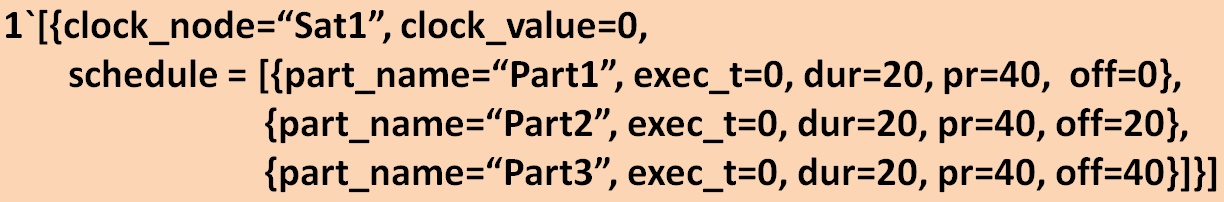
\includegraphics[width=\textwidth]{./img/clock}
	\caption{A Clock Token with Temporal Partitioning}
	\label{fig:clock}
\end{figure}

These extended data structure fields can be more easily manipulated and used by the model transitions during state changes, allowing for richer modeling concepts that would not be easily attainable using token representations provided by Timed Petri Nets. The ability to pack colored tokens with rich data structures also reduces the total number of colors required by the complete model. This quantitative measure directly influences the reduced size of the resultant state space. The downside of this approach to modeling is that we have to choose a time quantum. But in practical systems this is usually not a problem, as the low-level scheduling decisions are taken by an OS scheduler based on a time scale with a finite resolution. 

Secondly, modeling time as a token allows for smarter time progression schemes that can be applied to control the pace of simulation. If we did not have such control over time, the number of states recorded for this color token would eventually explode and itself contribute to a large state space. In order to manage this complexity, we have devised some appropriate \emph{time jumps} in specific simulation scenarios. 

If the rate at which time progresses does not change, then for a 1 msec time resolution, \emph{S} seconds of activity will generate a state space of size: $SS_{size} = \sum\limits_{i=1}^{S*1000} TF_{t_i}$ where $TF_{t_i}$ is the number of state-changing CPN transition firings between $t_i$ and $t_{i+1}$. This large state space includes intervals of time where there is no thread activity to analyze either due to lack of operation requests, lack of ready threads for scheduling, or due to temporal partitioning. During such idle periods, it is prudent to allow the analysis engine to \emph{fast-forward} time either to (1) the next node-specific clock tick, (2) the next global timer expiry event, or (3) the next activation of the node-specific temporal partition (whichever is earliest and most relevant). This ensures that the generated state space tree is devoid of nodes where there is no thread activity.

\begin{figure}[h]
	\centering
	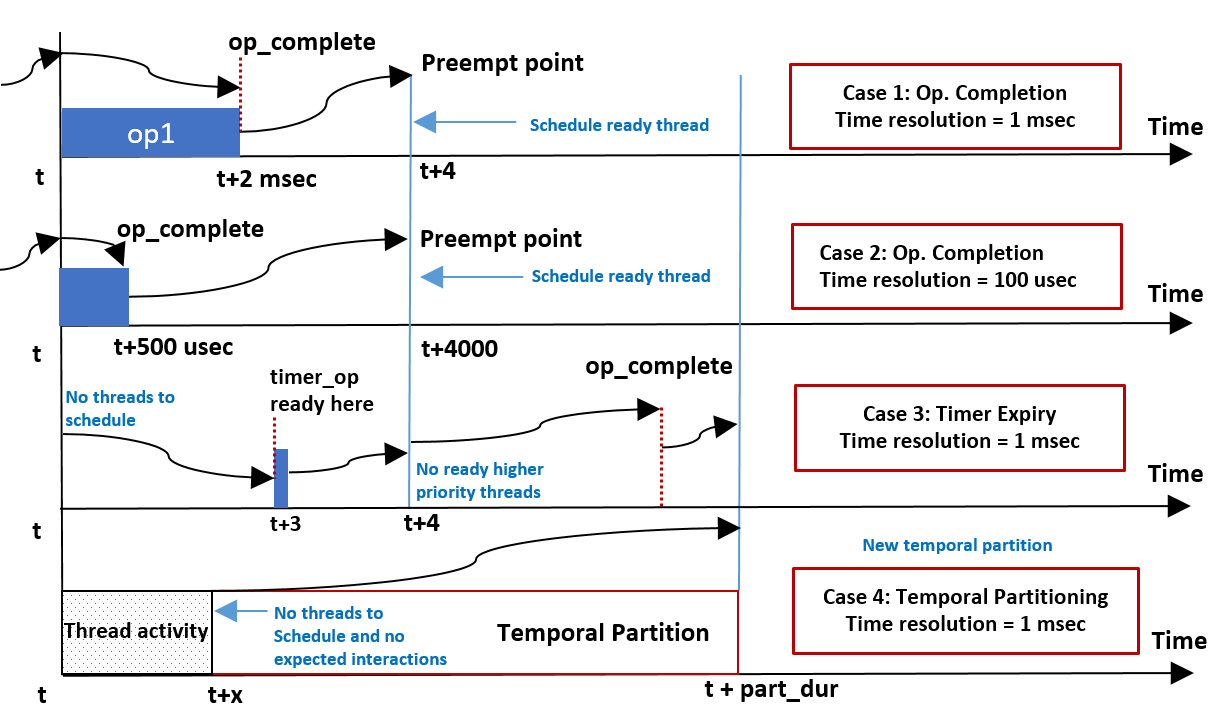
\includegraphics[width=\textwidth]{./img/time}
	\caption{Dynamic Time Progression}
	\label{fig:time}
\end{figure}

Figure \ref{fig:time} illustrates these time jumps using 4 scenarios. Assuming the scheduler clock ticks every 4 msec, Case 1 shows how time progression is handled when an operation completes 2 msec into its thread execution. At time t, the model identifies the duration of time left for an operation to complete. If this duration is earlier than the next preemption point, then there is no need to progress time in 1 msec increments as no thread can preempt this currently running thread till time t + 4 msec. Therefore, the \emph{clock\_value} in Figure \ref{fig:clock} progresses to time t + 2 msec, where the model handles the implications of the completed operation. This includes possibly new interactions and operation requests triggered in other components. Then, time is forced to progress to the next preemption point where a new candidate thread is scheduled. This same scenario is illustrated in Case 2 when the time resolution is increased to 100 usec instead of 1 msec. Notice that the number of steps taken to reach the preemption point are the same, showing how the state space doesn't have to explode simply because the time resolution is increased. Case 3 illustrates the scenario where at time t, the scheduler has no ready threads to schedule since there are no pending operation requests but at time t + 3 msec, a component timer expires, triggering an operation into execution. Since timers are maintained in a global list, each time the \emph{Progress\_Time} transition checks its firing conditions, it checks all possible timers that can expiry before the next preemption point. So, at time t when no threads are scheduled, the model immediately jumps to time t + 3. This scenario also shows that if the triggered operation does not complete before the preemption point \emph{and} there are no other ready threads or timer expiries that can be scheduled, the clock value jumps to the operation completion. It must be noted here that this case is valid only because the DREMS architecture we have considered uses a non-preemptive operation scheduling scheme. Lastly, Case 4 shows time jumps working with temporal partitioning. At some time t + x, the model realizes the absence of ready threads and does not foresee any interaction requests from other components, then it safely jumps to the end of the partition without stepping forward in 1 msec increments. This time progression directly shows how the state space of the system execution reduces while still preserving the expected execution order, justifying our choice of modeling time as a colored token using CPN. 

\subsection{Distributed Deployment} 
\label{distributed_deployment}

The second structural change to the analysis model is in how distributed deployments are modeled and simulated. Early designs on modeling and analysis of distributed application deployments \cite{kumar2014colored} included a unique token per CPN place for each hardware node in the scenario. Since the individual \emph{node} tokens are independent and unordered, there is nondeterminism in the transition bindings when choosing a hardware node to schedule threads in. For instance, if there are 2 hardware nodes in the deployment with ready threads on both nodes, then either node can be chosen first for scheduling threads leading to two possible variations of the model execution trace. Therefore the generated state space would exponentially grow for each new hardware node. In order to reduce this state space and improve the search efficiency, we have merged hardware node tokens into a single \emph{list} of tokens instead of a unassociated grouping of individual node tokens. This approach is inspired by the symmetry method for state space reduction \cite{Kristensen2000}.

\begin{figure}[h]
	\centering
	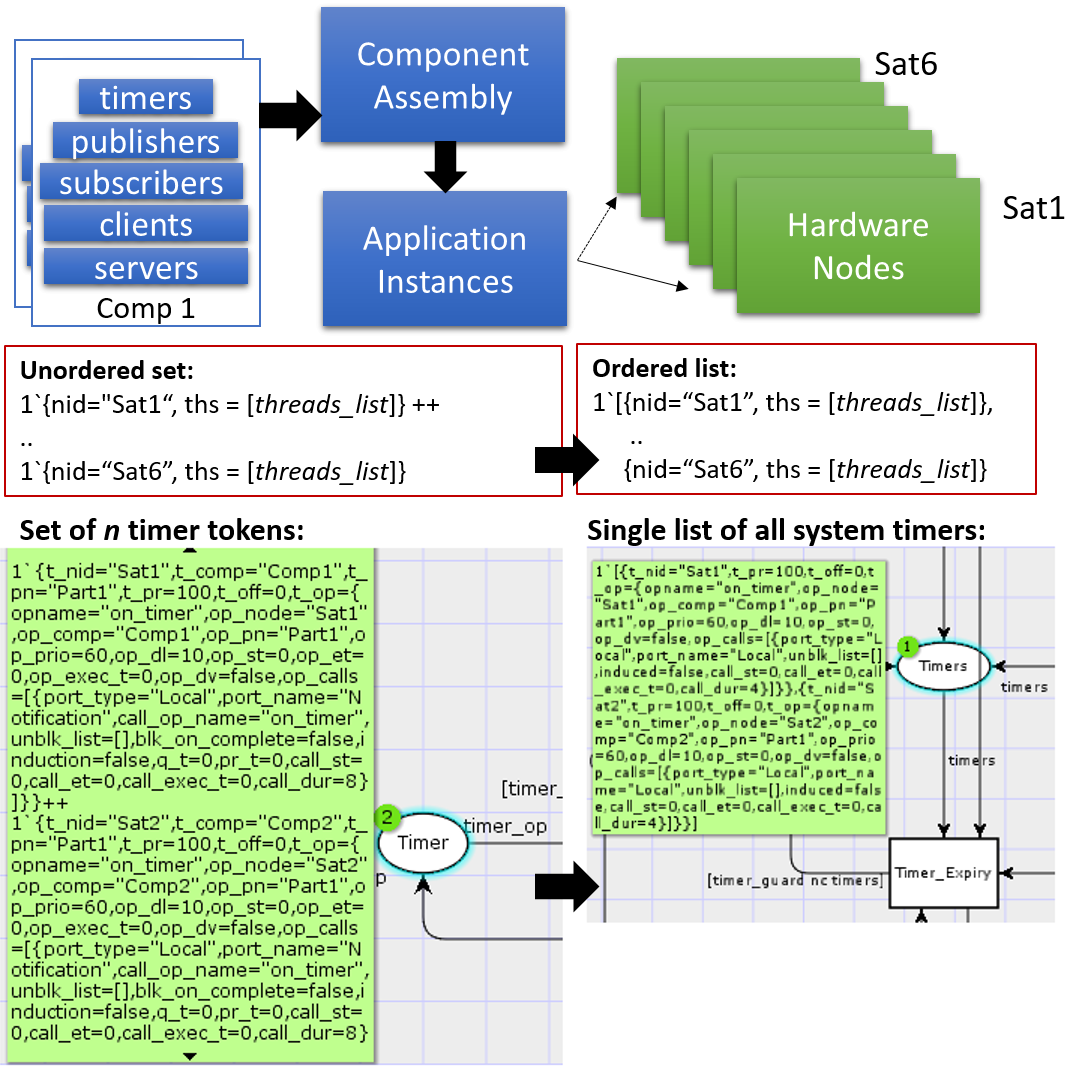
\includegraphics[width=0.8\textwidth]{./img/dd}
	\caption{Structural Reductions in CPN}
	\label{fig:dd}
\end{figure}

Figure \ref{fig:dd} illustrates this structural reduction. Consider a distributed deployment scenario with an instance of a DREMS application deployed on each hardware node, Sat1 through Sat6. Components \emph{Comp1} and \emph{Comp2} are triggered by timers, eventually leading to the execution of component operations (modeled as shown in Figure \ref{fig:ebnf}). If all the timer tokens in the system were modeled individually, the transition \emph{Timer\_Expiry} would non-deterministically choose one of the two timer tokens that are ready to expire at \emph{t=0}. However, if the timers are maintained as a single list, then this transition (1) consumes the entire list, (2) identifies all timers that are ready to expire, (3) evaluates the timer expiration function on all ready timers, (4) propagates the output \emph{operation} tokens to the relevant component message queues in a single firing. This greatly reduces the tree of possible transition firings and therefore the resultant state space. Also, if there is no non-determinism in the entire system, i.e., there is a distinct ordering of thread execution, then this model can be scaled up with instantiating the application on new hardware nodes with no increase in state space size. This is because all of the relevant tokens on all nodes are maintained as a single list that is completely handled by a single transition firing. 

An important implication of the above structural reduction is that the simulation of the entire system now progresses in synchronous steps. This means that at time 0, all the timers in all hardware nodes that are ready to expire will expire in a single step. Following this, all operations in all component message queues of all these nodes are evaluated together and appropriate component executor threads are scheduled together. When these threads execute, time progresses as described in Section \ref{handling_time}, moving forward by the minimum amount of time that can be fast-forwarded.

\newpage
\section{Scalability: Investigating Advanced State Space Analysis Methods}

The main disadvantage of using state spaces for analysis is the state explosion problem: even relatively small systems may have an astronomical number of reachable states, and this is a seriou limitation to the use of state space methods in analysis of real-life systems. This has led to the development of many different reduction methods for alleviating the state explosion problem. Examples of such reduction techniques include partial order reduction methods \cite{peled1993all, valmari1990stubborn, wolper1993partial}, and the symmetry method \cite{jensen1996condensed}. Reduction methods represent the full state space in a compact, condensed form or represent only a subset of the full state space. The reduction is done such that the answer to the verification questions can still be determined from the reduced state space. 

The scalability of the DREMS timing analysis CPN has been improved using the symmetry method, as described in the previous section. Instead of reinventing any state space reduction methods, the ASAP \cite{ASAP} analysis platform is used to effectively apply existing advanced state space analysis methods on the DREMS analysis model with no additional changes. In ASAP, the CPN analysis model is imported as such and integrated into a \emph{verification project}. ASAP provides a platform on which to choose a variety of analysis parameters e.g. the type of graph traversal (depth-first, breadth-first etc.) and any analysis technique e.g. sweepline method as relevant. 

\begin{table}[h]
	\centering
	\caption{Scalability Testing with CPNTools and ASAP -- A bounded state space covering 10 hyperperiods of component interactions is generated}
	\label{tbl:scalability}
	\begin{tabular}{|c|c|c|c|c|c|c|}
		\hline
		\textbf{Tool} & \textbf{\begin{tabular}[c]{@{}c@{}}Test\\ Case\end{tabular}} & \textbf{\begin{tabular}[c]{@{}c@{}}Number of \\ Embedded\\ Nodes\end{tabular}} & \textbf{\begin{tabular}[c]{@{}c@{}}Temporal \\ Partitions \\ per\\ Node\end{tabular}} & \textbf{\begin{tabular}[c]{@{}c@{}}Threads\\ per \\ Partition\end{tabular}} & \textbf{\begin{tabular}[c]{@{}c@{}}Size of \\ State\\ Space\end{tabular}} & \textbf{\begin{tabular}[c]{@{}c@{}}Generation \\ Time\end{tabular}} \\ \hline
		CPNTools      & 1                                                            & \textbf{5}                                                                     & 2                                                                                     & 1                                                                           & 180                                                                       & 0.981 s                                                             \\ \hline
		CPNTools      & 2                                                            & \textbf{2}                                                                     & 5                                                                                     & 5                                                                           & 124,469                                                                   & 14.1 m                                                              \\ \hline
		CPNTools      & 3                                                            & 5                                                                              & 5                                                                                     & 4                                                                           & 485,552                                                                   & 36.5 m                                                              \\ \hline
		ASAP          & 3                                                            & 5                                                                              & 5                                                                                     & 4                                                                           & 144,861                                                                   & 495.147 s                                                           \\ \hline
	\end{tabular}
\end{table}

Using the CPN Tools' built-in state space analysis tool, a bounded state space was generated reaching up-to 10 hyperperiods of component thread activity on a 100-component example. This bounded generation took 36 minutes on a typical laptop. The goal with using ASAP is to evaluate the effectiveness and utility of advanced state space reduction techniques that can be readily applied on any Colored Petri net, such as the DREMS analysis model. With no changes to the model, the model is analyzed in ASAP for system-wide deadlocks in under 10 minutes. Table \ref{tbl:scalability} summarizes these results. It must be noted that the size of the state space is reduced partly due to temporal partitioning itself. As described using Figure \ref{fig:SSScreenshot}, the branching nature of the state space graph is dependent on (among other factors) the number of "ready" equal-priority component executor threads. With temporal partitioning, this number reduces down to a fraction of the total number of components. Without temporal partitioning, if all 100 threads are theoretically ready to execute, then the state space would be in the millions and the state explosion would make any analysis intractable. So, it is observed that though tools like ASAP help alleviate the state explosion and make state space generation occur in much faster rates, the DREMS timing analysis model is still affected by this explosion in very large-scale systems with potentially thousands of components.


%The tool provides for several search algorithms and state space reduction techniques such as the \emph{sweep-line method} \cite{Christensen2001} which deletes already visited state space nodes from memory, forcing on-the-fly verification of temporal properties. The main advantage of such techniques is the amount of memory required by the analysis to verify useful properties for large models. 

\if 0

%The sweep line method for state space reduction is used to check for important safety properties such as lack of deadlocks, timing violations etc. using user-defined model-specific queries. Practical results enumerated in \cite{Christensen2001} show improvements in time and memory requirements for generating and verifying bounded state spaces. The method relies of discarding generated states on-the-fly by performing verification checks during state space generation time. Any state that does not violate system properties can be safely deleted. Another advantage of this method compared to similar reduction methods such as bit-state hashing \cite{CPN_Bitstate_Hashing} is that a complete state space search is guaranteed. 

%These methods were evaluated on our CPN analysis method and the results were presented in \cite{SEUS}. We used a large and diverse 100 component-based application for our testing. Using the CPN Tools' built-in state space analysis tool, a bounded state space of thread activity was generated. The state space generation took 36 minutes on a typical x86 laptop. We imported the same CPN analysis model onto ASAP and performed on-the-fly verification checks for lack of dead states in the analysis model for the same bounded state space. The on-the-fly verification, without any graphical interface overheads, took less than 10 minutes to compute a lack of system-wide deadlocks. It must be noted here that this improved result is due to not only because of the efficient state space search but also because of symmetry-based structural reduction discussed in the previous section.

%In order to illustrate the utility of such state space reduction techniques, we consider a large-scale deployment. Figure \ref{fig:gm} shows the generated CPN model for a domain-specific DREMS application. This is a scaled-up variant of several satellite cluster examples we have used in previous publications \cite{DREMS13Software, kumar2014colored}. The example consists of a group of communicating satellites hosting DREMS applications. The component assembly for this application consists of 100 interacting components distributed across 10 computing nodes, many of which are triggered by infrastructural timers. Notice in Figure \ref{fig:gm} how there is only one token in each of the main CPN places, as described in Section \ref{distributed_deployment}. All of the component timers are appended to the list maintained in \emph{Timers} place. Similarly, all node-specific clock tokens are maintained in place \emph{Clocks}.  

%At time \emph{t=0}, before the simulation is kicked off, the transition \emph{Establish\_Order} generates the powerset of thread execution orders that are possible given the configuration of the clock token. This may be a potentially large set depending on the number of threads of equal priority in each partition. Once this tree of possible orders is established, the complete set of timers that are ready to expire are evaluated. Each timer expiry manifests as an operation request and each callback operation modeled using the grammar shown in Figure \ref{fig:BL_Model}. Once the operations are ready to execute, the highest priority component thread with a pending operation request is chosen for execution. This thread scheduling happens on all hardware nodes. When each thread executes, new interactions may occur as a consequence of the execution. For instance, if a component thread executes a timer operation in which the component publishes on a global topic, the consequence of this action would include a set of callback operation requests on all components that contain subscribers to that global topic. Lastly, all running threads are evaluated to identify the minimum amount of time that can be safely fast-forwarded in each node. If the running component threads are independent or symmetrical, then the maximum possible time progression is up to the end of the temporal partition. Note here that temporal partition in the deployment can be set to an empty list which simply removes the  partitioning constraint and treats all component threads on a node as candidate threads for execution. The above sequence of transitions repeat for as long as there is a timer expiry, a pending operation request or an unfinished component interaction. 

\begin{figure}[h]
	\centering
	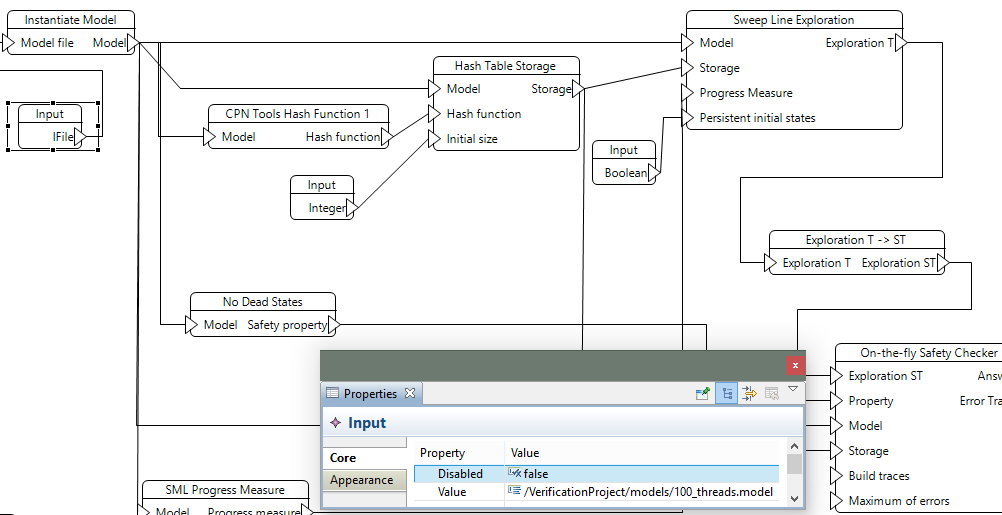
\includegraphics[width=\textwidth]{./img/sl}
	\caption{Sweep-Line Method}
	\label{fig:sl}
\end{figure}

%Using the CPN Tools' built-in state space analysis tool, a bounded state space was generated reaching up-to 20 hyperperiods of component thread activity. This bounded generation took 36 minutes on a typical laptop. Our goal with such an example is to evaluate the effectiveness and utility of state space reduction techniques with respect to speed and memory usage. Figure \ref{fig:sl} shows a simple block diagram of the sweep-line method as configured in ASAP. Performing on-the-fly verification checks for lack of dead states in the analysis model, results indicate lack of system-wide deadlocks due to blocking behaviors triggered by RMI-style synchronous peer-to-peer interaction patterns. Figure \ref{fig:ds} shows analysis results obtained from a \emph{Verification Job} executed in the tool. Notice the on-the-fly verification taking less than 10 minutes to perform deadlock checks on this sample deployment. Using the \emph{Palette} in ASAP, several standard ML (SML) user queries can be created to check for domain-specific properties. 

\begin{figure}[h]
	\centering
	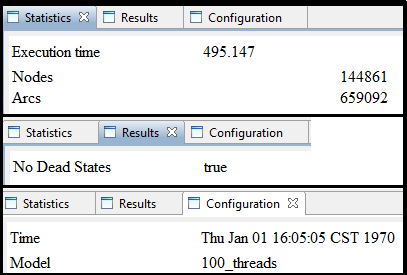
\includegraphics[width=0.6\textwidth]{./img/asap}
	\caption{Dead States Checking in a Component-based application}
	\label{fig:ds}
\end{figure}

%It must be noted here that this improved result is due to not only because of the efficient state space search but also because of symmetry-based structural reduction discussed in the previous section. If not for this reduction, the state space search requirements would exponentially grow for each new hardware node added to the deployment. 
\fi